% article example for classicthesis.sty
\documentclass[11pt,a4paper]{scrartcl} % KOMA-Script article 
\usepackage[nochapters,eulermath]{classicthesis} % nochapters
\pdfoutput=1

% Packages here
\usepackage{lipsum}
\usepackage{graphicx}
\usepackage[left=1.5in,right=1.5in,top=1in,bottom=1in]{geometry}
\usepackage[natbibapa]{apacite}
\setcitestyle{notesep={: }}
\usepackage{listings}
\lstset{basicstyle=\ttfamily}
\usepackage{fancyvrb}
\usepackage{gb4e}
% this next command fixes some bug in gb4e
\noautomath
\usepackage{float}
\usepackage{adjustbox}
\usepackage{amsmath}

\newcommand{\bce}{\textsc{bce}\ }
\newcommand{\ce}{\textsc{ce}\ }

\newenvironment{myverb}{%
 \VerbatimEnvironment
 \begin{adjustbox}{max width=\linewidth}
 \begin{BVerbatim}
  }{
  \end{BVerbatim}
 \end{adjustbox}
}

\begin{document}
\title{\rmfamily\normalfont\textsc{A Large-Corpus Investigation of Latin Verb Order to 800ce}}
\author{\phantom{xxx}\\\textsc{Ben Nagy}\\\small{\texttt{benjamin.nagy@adelaide.edu.au}}}
\date{\normalsize{November 8, 2018}}

\maketitle

\begin{abstract}
\noindent I designed and implemented computational techniques to analyse 1178 written works of Latin, dated between $\sim$230\bce and 800\ce (a total of 1.87 million sentences) with respect to OV and VO word order---the largest such study yet. The analysis was carried out with probabilistic methods, but exhibits a low estimated rate of type 1 errors (false positives). I demonstrate modest evidence for a general trend from OV to VO word order up to 425\textsc{ce}. After this point there is insufficient evidence to support a correlation between date of authorship and word order. The analysis also shows extreme synchronic variation. This is visible not only among authors, but even within the works of a single author. There is evidence to suggest that this synchronic variation in OV/VO `style' increases in later authors. This variation calls into question any conclusions drawn from comparative studies using small sample sizes.\\
\phantom{xxx}\\
\noindent\textit{Keywords: Latin, SOV, language change, computational linguistics, corpus linguistics, NLP}
\end{abstract}


\section{Introduction}

Much has been said about the evolution of Latin, the ancestor of `Romance',
\footnote{It is not at all clear that such a language ever existed, and, if it did, that it was ever called Romance. On this, see \textit{Latin and the Romance Languages in the Early Middle Ages} (\cite{wright}) generally.}
and eventually, modern languages like Spanish, French and English (at least after 1066). In this paper I focus specifically on one aspect: the hypothesis that Latin evolved from a language that was verb-final, and SOV in particular, to one that was SVO. \cite{linde} is the seminal paper approaching this from a statistical point of view, arguing that Classical Latin was verb-final. The definitive modern work, however, is \cite{pinkster}. Pinkster considers analyses by Linde, as well as Koll, his own (1984) research and that of Metzeltin. His conclusion, which has not since been significantly challenged, was that ``there is no reason for assuming a SOV word order for Classical Latin, nor is there one for assuming a SVO order by \textsc{ad} 400" \cite[80]{pinkster}.

It is striking, however, that this debate has been conducted based entirely on statistics extracted from woefully small samples. Linde manually analysed excerpts of larger works, eg Livy 30.30--45, Tacitus \textit{Germ.} 1--37 and Sallust \textit{Cat.} 1--36 \cite[154]{linde}. The studies cited in Pinkster (1991: 72) analyse a few hundred sentences at most, from less than twenty works in total. The statistical significance of these samples, considering the size of the Latin corpus available to us, is virtually nil---and yet such approaches are still deployed in modern scholarship. \cite{blake} uses a similar summary, again based on subsets of just five works, to claim that it is ``strikingly clear that VO was the favoured syntactic pattern for whatever was being spoken (Vulgar Latin?) by the fourth century" \cite[223]{blake}. This claim owes more to confidence than to evidence. In this study I aim to address this lack of data. While some of the findings may, on their face, support or refute previous hypotheses about the development of written Latin word order, it is not my intent to to take a position. The key contribution of this paper is the development of tools and techniques to collect and analyse data on a much larger scale than any previous study. My analysis is designed to be replicated or extended. I publish (\cite{ovvo}), alongside this paper, the complete corpus of data, all of the software tools that I developed and the analysis script for the R statistics environment (\cite{r}).

\section{Methods}

\subsection{Designing the Study}
The aim of the project was to perform a large-scale analysis of OV/VO on written texts. To this end, a number of restrictions were made. The project aims only to analyse OV/VO, and does not include any consideration of the position of the subject (subject position is complicated in Latin, because subject information is often included in the verb). Sentences were only analysed if they contained a qualifying transitive verb---one that was considered likely to take a nominal direct object (DO). These verbs were selected by considering the 1000 most common words in Latin (\cite{vocab}), and manually selecting transitive verbs that seemed suitable. Verbs of thinking and feeling, for example, often take a phrase in complement instead of a DO, which would have complicated the analysis. The final list contained 171 qualifying verbs. Latin poetry was not analysed, because of its tendency to distort word order to conform to metre.\footnote{Informally, the analysis was also run with the poetry included. There was no substantial change to any of the conclusions.} The final consideration was the selection of a terminus date. 800\ce was chosen for two reasons---first, since the earliest texts are those of Plautus around 235\textsc{bce}, 800\ce yields a fairly neat window of one millennium or so. Second, it aims to avoid complications due to texts that might have been affected by the Carolingian Renaissance, and, in particular, Charlemagne's linguistic reforms.

\subsection{Collecting and Cleaning the Data}
I obtained\footnote{%
I would like to extend my thanks to Dr P. Roelli, the author and maintainer of the \textit{Corpus Corporum} project for his assistance in acquiring these corpora, as well as useful feedback on the project.}
three corpora from the \textit{Corpus Corporum} (\cite{CC}): The \textit{Patrologia Latina}, a well known collection of over five thousand ecclesiastical works dated from 230--1617\textsc{ce}, \textit{Latinitas Antiqua}, a collection including most of the Classical Latin corpus,\footnote{One notable exception was the \textit{Natural History} of Pliny the Elder, a significant work, which was added manually to the analysis corpus.} and \textit{Monumenta}, a selection of seventy works from the \textit{Monementa Germaniae Historica}. In total, this amounted to 5544 documents in XML format. The documents were then `cleaned'%
\footnote{For full details of the cleaning process, consult the project source code repository (\cite{ovvo}). Examples include removing parenthetical references, especially to biblical passages ([Job X.XIV]), removing Arabic line numbers that were included by the original OCR process, and removing or normalising a bewildering variety of punctuation marks.
}
and converted to plain text format. After discarding files whose date could not be determined, this left 3226 files. These were further restricted to reject files written after 800\textsc{ce}, works by known Classical poets and works by other authors whose title included the word \textit{carmina} (poems). After the cleaning process, the input to the analysis phase was 1289 text files containing one sentence per line, totalling 1.87 million sentences. These sentences are not confined to Latin text---many contain English (from glosses or commentary), French or, fairly commonly, Ancient Greek. Of the initial 1.87 million sentences, around 780 thousand contain at least one of the qualifying transitive verbs.

\subsection{Performing the Syntactic Analysis}
For in-depth technical details of the analysis, the reader should consult the source code (\cite{ovvo}). In this section I will provide an overview. To perform the required analysis, the software must automatically determine the `lemma' (root lexical entry) and part of speech (POS) of each word. This then allows transitive verbs to be positionally related to nouns in accusative case. However, one of the problems when automatically analysing Latin text is that surface forms often collide, yielding multiple possible combinations of lemma+POS. To address this issue, the core of the analysis code was an interface to the software tool ``Collatinus---Latin Lemmatizer, Morphological Analyzer and Scansion" (\cite{collat}).%
\footnote{Collatinus is interactive desktop software, not a bulk analyser, but it offers a `TCP' interface that can be used by other programs. The bulk analysis tools used in this study were developed by the author.}
Collatinus includes a `statistical tagger' which not only returns all possible combinations of lemma+POS, but also assigns a probability to each combination. For example, in Figure \ref{fig:cadam}, note that the two possible lemma+POS combinations for \textit{cadam} are listed with different probabilities: 90.18\% for \textsc{1s.fut.ind.act} and 9.8\% for \textsc{1s.pres.subj.act}

\begin{figure}[H]
\centering
\caption{Raw output from my Collatinus-based POS tagger for \textit{cadam}}
\label{fig:cadam}
\phantom{xxx}
\begin{Verbatim}[fontsize=\footnotesize]
[
    `cadam',
    `to fall, sink, drop, plummet, topple; to be slain, die; to end, cease, '
    `abate; to decay;',
    `cadam future indicative active 1st singular (v1  : 0.901807)'
],
[
    `cadam',
    `to fall, sink, drop, plummet, topple; to be slain, die; to end, cease, '
    `abate; to decay;',
    `cadam present subjunctive active 1st singular (v21 : 0.0981932)'
]
\end{Verbatim}
\end{figure}

\noindent The probabilities assigned by Collatinus are based on occurrences in the LASLA corpus (\cite{lasla}), a collection of around 1.6 million words which have been hand-glossed with syntactic information. The probabilistic tagger will, of course, make many mistakes---but this is not as much of a problem as it may seem. For verbs, as long as they are in the active voice, the mood or tense does not greatly affect the analysis---if a tree falls in the forest, whether in future tense or present subjunctive, it is still the subject of the verb `to fall'. For nouns, the analysis code considers any surface form that \textit{might} be a noun in accusative case, so it is not subject to errors based on probabilistic tagging. This approach is intended to reduce false positives (by increasing the number of false negatives), and is discussed in more depth below. Finally, it is possible that the software might tag something as a verb when it is really, for example, a noun (not impossible in Latin by any means---\textit{canis} can be both dog.\textsc{nom.s} and the verb sing.\textsc{2s.pres.ind.act}). This is unlikely, but is a source of potential errors.

The next problem in the analysis phase is attempting to determine the grammatical relationships between qualifying (transitive) verbs and their DOs. Latin sentences can be very complex, with deeply nested clauses, and DOs can be quite distant from their verbs. The `correct' approach would be to completely parse the sentence and build a sentence tree. However, this is presently intractable with automatic approaches.%
\footnote{It is also likely to remain intractable. Any such system would likely require accurate POS tagging as a pre-requisite; in itself a problem with no good automatic solutions.}
In my analysis, I make a compromise by considering a small `slice' of words around each verb. For each qualifying verb, the analysis code looks ahead and behind up to three words, and marks any words which \textit{might} be in accusative case. In many cases, the analysis can be improved by `stopping' at commas, since most manuscript editors use commas to delineate clause boundaries. This is best illustrated with a few examples. During the analysis, I collected a random sample of around one percent of the analysis decisions so that the accuracy of the analysis could be assessed; these examples are drawn from that sample. In figure \ref{fig:slice1}, \textit{habetis} is the verb. The traversal backwards stopped at the comma (before \textit{qui}), and traversal forwards stopped at the accusative noun \textit{inimicum} `enemy.\textsc{acc.sg}'. Since a possible DO was only found on one side of the verb, this sentence was classified VO. Although, in this case, the parser is correct, it is definitely possible for false positives to occur. For example, suppose \textit{inimicum} were not the true object, but instead the DO was far before \textit{habetis} and outside our three-word slice---that would result in a misclassification.

\begin{figure}[H]
\centering
\caption{Sentence analysis example}
\label{fig:slice1}
\phantom{xxx}
\begin{Verbatim}[fontsize=\small]
SENTENCE:   Deponite ferrum, qui non <<habetis>> inimicum.
SLICE:      qui non <<habetis>> [inimicum]
RESULT:     VO
\end{Verbatim}
\end{figure}

\noindent In Figure \ref{fig:slice2}, no accusative noun was found in the slice, so the sentence was classified as NONE (not counted as a result for VO or OV). 

\begin{figure}[H]
\centering
\caption{Sentence analysis example}
\label{fig:slice2}
\phantom{xxx}
\begin{myverb}[fontsize=\small]
SENTENCE:   Sed cum facis conuiuium, uoca pauperes, debiles, claudos, 
            caecos; et beatus eris, quia non <<habent>> unde retribuant tibi.
SLICE:      quia non <<habent>> unde retribuant tibi
RESULT:     NONE
\end{myverb}
\end{figure}

\noindent This example demonstrates, in some senses, a failure of this kind of analysis. As we can see in glossed example \ref{ex1}, the object of \textit{habent} is the phrase `a way to reward you', but there is no direct object:

\begin{exe}[fontsize=\small]
\ex\label{ex1}
\gll quia non habent unde retribuant tibi \\
because not have.\textsc{3p.pres.ind.act} from-where reward.\textsc{3p.pres.subj.act} you.\textsc{dat.sing}\\
\trans `because they have no way to reward you'
\end{exe}

\begin{figure}[H]
\centering
\caption{Sentence analysis example}
\label{fig:slice3}
\phantom{xxx}
\begin{Verbatim}[fontsize=\small]
SENTENCE:   in saecula saeculorum <<laudabunt>> te.
SLICE:      [saecula] saeculorum <<laudabunt>> [te]
RESULT:     BOTH
\end{Verbatim}
\end{figure}

\noindent Finally, in Figure \ref{fig:slice3}, we see a type 2 error (false negative). This sentence is glossed as example \ref{ex2}. Because \textit{saecula} has the same surface form for \textsc{nom.pl} and \textsc{acc.pl}, the analyser treats it as a possible object (the true DO is \textit{te}), and cannot decide whether to classify the sentence as OV or VO:

\begin{exe}[fontsize=\small]
\ex\label{ex2}
\gll in saecula saeculorum laudabunt te \\
in ages.\textsc{nom.pl} ages.\textsc{gen.pl} praise.\textsc{3p.fut.ind.act} you.\textsc{acc.sg}\\
\trans `they will praise you forever and ever'
\end{exe}

\noindent Using the method described, around 64\% of 780 thousand qualifying sentences were `successfully' processed (yielded a conclusive result of VO or OV), about half a million sentences. Although some level of error is to be expected, it is difficult to estimate the rate of false positives. I analysed a sample of two hundred sentences by hand and found no misclassifications. Two hundred from half a million may not seem very convincing, but in fact it is fairly significant---the error rate is unlikely to be zero, but it is probably less than 5\%.\footnote{%
If I made no errors while checking, and the real error rate were 5\%, then the probability of seeing no errors in a sample of 200 results is around 1 in 25000.
} After the analyser has run on every sentence for a given work, it produces a human-readable output file with the summary results, as shown below:

\begin{figure}[H]
\centering
\caption{Analysis output from Columella's \textit{De Re Rustica}}
\label{fig:columella}
\phantom{xxx}
\begin{myverb}[fontsize=\footnotesize]
{
  "author": "Columella",                        
  "date": 57.65,        # dates are randomly jittered. This makes it easier to 
                        # distinguish different entries on a scatterplot and
                        # has negligible effect on the statistical analysis
  "file": "./cps5/Columella_De-re-rustica.xml",
  "lines": 7577,        # sentences in the work
  "qual": 1912,         # sentences containing a qualifying transitive verb
  "sov": 990,           # sentences classified as OV
  "svo": 224,           # VO
  "none": 457,          # ...etc
  "both": 241,
  # Internal tracking information for files produced in the cleaning passes
  "pass1": "pass1/6c161f3b24365b10fb606ab32965b875d024c08d11a22e0a1363668dfae5f9e8.txt",
  "pass2": "pass2/0d18895be2f71df2039b3090a955fc1e2fad33b4ee93c1f4a5f78872656fb001.txt",
  "sample": [
    [
      "VERB: sequor - to follow; to escort/attend/accompany",
      "SENTENCE: <<Sequitur>> ut tempora quoque subigendi arui praecipiamus",
      [
        "<<Sequitur>>",
        "ut",
        "[tempora]"
      ]
    ],
    [...many entries skipped...]
  ],
  "title": "De re rustica",
}
\end{myverb}
\end{figure}

\noindent Finally, these files are then processed in bulk to produce a CSV summary, ready for analysis with a higher level software package. For this study, the further analysis was performed with ``R Studio", a widely used open-source statistics processing environment. Of the 1289 files, I discarded 111 files with less than ten qualifying sentences, since percentage results based on such small numbers are unreliable.

\section{Results}

In this section,  I discuss the results of the statistical analysis. It is important to bear in mind that statistical analysis can provide evidence of correlation (the use of OV word order decreases as time goes on), but not causation (word order changed \textit{because} time went on). To begin, figure \ref{fig:sp_empty} shows the raw results. Each dot is a single work, with longer works being drawn both larger and darker. 

\begin{figure}[H]
    \caption{A visualisation of the data (longer works drawn larger and darker)}
    \label{fig:sp_empty}
    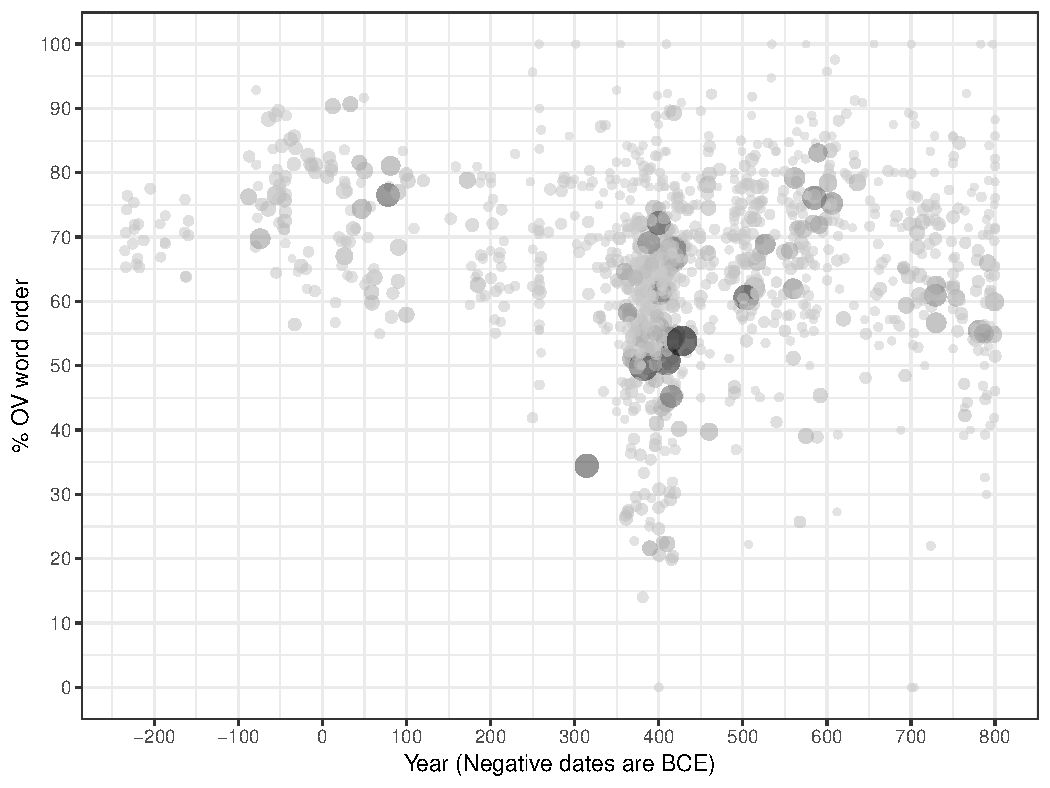
\includegraphics[width=\textwidth]{sp_empty.pdf}
\end{figure}

\noindent We can make several qualitative observations immediately. It is clear from the data that the idea of a  `standard' written word order, even in the Classical period, is strongly challenged. We also note the dense band of works near the turn of the fifth century \textsc{ce}, and the extreme variation in that section. In particular, the distinct cluster of works between 20--30\% OV around 400\ce is interesting---these are mainly books of the Vulgate Bible, produced by Saint Jerome, discussed further below. Statistically, the data appears very `rich'---there is no strong visual evidence of a trend from OV to VO in relation to time. We can see that there are changes happening, but (as we also know from our historical evidence) time is not the only factor at work. To frame this in statistical terms, we can attempt to fit a linear model (weighted by the size of the works),
\footnote{For the technically minded, or those who are interested in replicating or extending these results, the accompanying source code repository contains \texttt{latin.R}, a complete record of the analysis process.}
 to test the hypothesis that date is correlated with word order. This regression is shown in figure \ref{fig:sp_single_lm}, and the numerical results of the analysis in figure \ref{fig:r_single}.

\begin{figure}[H]
    \caption{Weighted linear regression}
    \label{fig:sp_single_lm}
    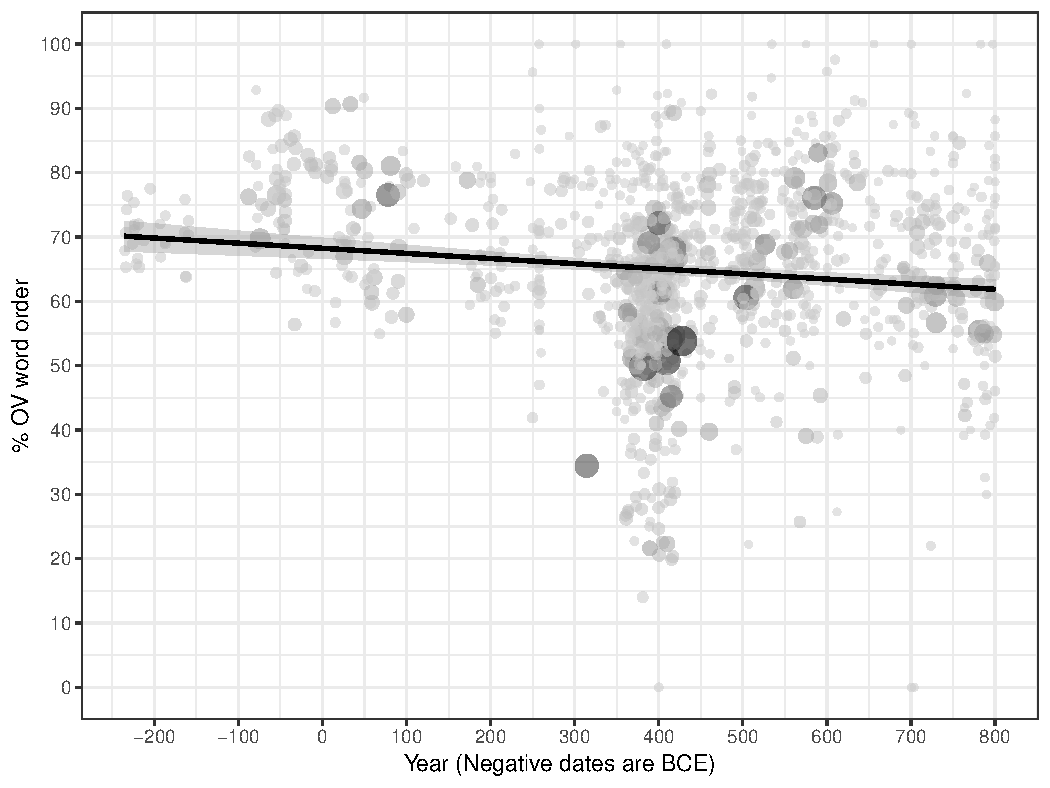
\includegraphics[width=\textwidth]{sp_single_lm.pdf}
\end{figure}

\begin{figure}[H]
\centering
\caption{R summary output for the weighted linear regression}
\label{fig:r_single}
\phantom{xxx}
\begin{Verbatim}[fontsize=\small]
Call:
lm(formula = pct_ov ~ date, data = analysis, weights = log(vo + ov))

Weighted Residuals:
     Min       1Q   Median       3Q      Max 
-123.172  -13.998    2.992   21.521   71.881 

Coefficients:
             Estimate Std. Error t value Pr(>|t|)    
(Intercept) 68.255973   0.819093  83.331  < 2e-16 ***
date        -0.007974   0.001751  -4.553 5.83e-06 ***
---
Signif. codes:  0 ‘***’ 0.001 ‘**’ 0.01 ‘*’ 0.05 ‘.’ 0.1 ‘ ’ 1

Residual standard error: 29.75 on 1176 degrees of freedom
Multiple R-squared:  0.01732,   Adjusted R-squared:  0.01649 
F-statistic: 20.73 on 1 and 1176 DF,  p-value: 5.829e-06
\end{Verbatim}
\end{figure}

\noindent There are two key things to note, here. First, the `trend' is almost non-existant, indicating a change from OV toward VO of around 8\% over 1000 years. The second is the ``R-squared" statistic---a value of 0.017 indicates (broadly speaking) that only about 2\% of the observed change in OV\% can be explained by the change in date. In statistical terms, this model is completely inconclusive. However, through `qualitative analysis', (ie by staring at the raw data in figure \ref{fig:sp_empty}) it seems like there \textit{is} an observable trend up until the fifth century, which is compatible with the historical narrative. In data with a `break', a point where some new factor came into play, it is common to fit a `piecewise' linear model. This effectively treats the data as two sets, and applies a linear regression to each piece. In our case, although our `break' seems to occur somewhere between 300\ce and 500\textsc{ce}, it is not clear exactly where. To resolve this, I tried a regression with a break at every year in that two hundred year interval, and plotted the `mean squared error', which is a measure of how well the model fits the data. This process indicated that the best year to break is 425\textsc{ce}, although several years around 420 are almost as good. This is reflected in figure \ref{fig:sp_mse}.

\begin{figure}[H]
    \caption{Selecting the date for piecewise regression}
    \label{fig:sp_mse}
    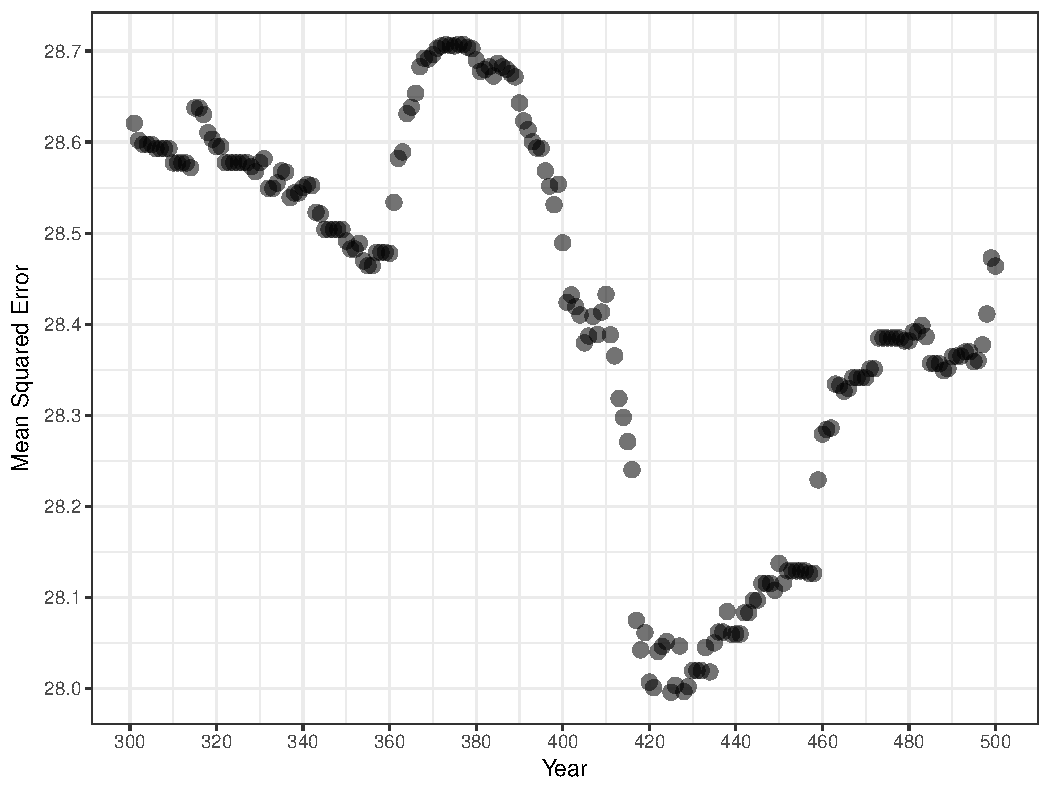
\includegraphics[width=\textwidth]{sp_mse.pdf}
\end{figure}

\noindent The next step was to perform the piecewise regression, shown in figure \ref{fig:sp_piecewise_lm}.

\begin{figure}[H]
    \caption{Piecewise linear regression, broken at 425\ce}
    \label{fig:sp_piecewise_lm}
    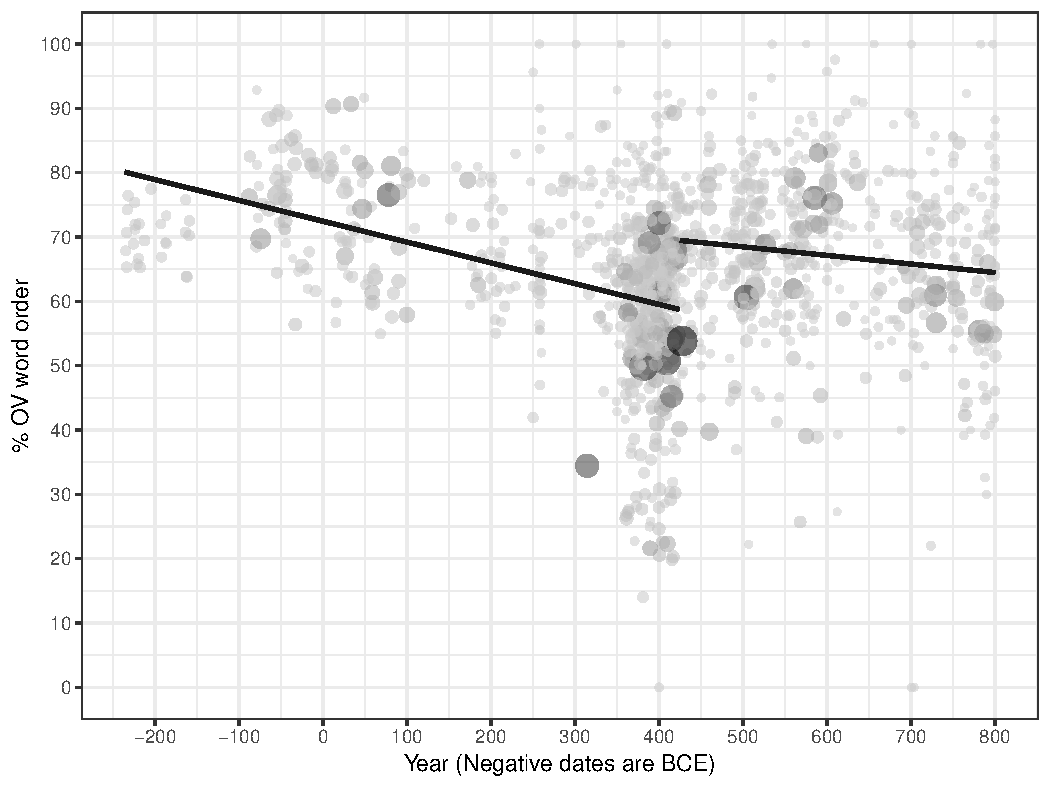
\includegraphics[width=\textwidth]{sp_piecewise_lm.pdf}
\end{figure}

\noindent Now, looking at the statistical results for the period up to 425\textsc{ce}, the picture is quite different (figure \ref{fig:r_piece1}). This data shows modest evidence for a real correlation between date and OV\% (an R-squared value of 0.1677 is fairly reasonable for data this messy). The statistics for the period after 425\ce (not shown) still have a very weak R-squared value; there is no evidence there to support the hypothesis that word order is changing over time.

\begin{figure}[H]
\centering
\caption{R summary output for the piecewise regression up to 425\ce}
\label{fig:r_piece1}
\phantom{xxx}
\begin{Verbatim}[fontsize=\small]
Call:
lm(formula = pct_ov ~ date, data = subset(analysis, date < cut.wts), 
    weights = log(vo + ov))

Weighted Residuals:
     Min       1Q   Median       3Q      Max 
-112.668  -14.741    4.015   20.339   81.260 

Coefficients:
             Estimate Std. Error t value Pr(>|t|)    
(Intercept) 72.456736   0.927205   78.14   <2e-16 ***
date        -0.032348   0.002805  -11.53   <2e-16 ***
---
Signif. codes:  0 ‘***’ 0.001 ‘**’ 0.01 ‘*’ 0.05 ‘.’ 0.1 ‘ ’ 1

Residual standard error: 29.34 on 660 degrees of freedom
Multiple R-squared:  0.1677,    Adjusted R-squared:  0.1664 
F-statistic:   133 on 1 and 660 DF,  p-value: < 2.2e-16
\end{Verbatim}
\end{figure}

\noindent In Pinkster's (1991) examination of previous studies on SVO word order, he noted that despite the fact that ``the samples used in most of these studies are very limited and the numbers of appropriate sentences very low", ``the most significant aspect [of the data] is the variety" \cite[71--2]{pinkster}. In this study I have examined orders of magnitude more data, but come to the same conclusion. Not only do different authors display synchronic variation, but individual authors can dramatically vary their style. This, as Pinkster notes (1991: 72) argues against a basic syntactic order. It is interesting, however, that the magnitude of this per-author variation does seem to increase after the Classical period. In figures \ref{fig:author_sd_least} and \ref{fig:author_sd_most}, I summarise the authors with the least and most standard deviation (a statistical measure of variability) of OV\%:
\begin{figure}[H]
\caption{Author OV variation---5 least variable}
\label{fig:author_sd_least}
\phantom{x}
\centering
\begin{tabular}{ | l | c | c | c | c | c |}
\hline
Author & Std. Dev. & Min OV\% & Max OV\% & Works & Avg. Date\\
\hline\hline
Titus Livius & 1.922 & 79.39 & 85.69 & 13 & -13 \\
Horatius Flaccus & 2.145 & 61.59 & 66.67 &  5 &  -23 \\
Prudentius & 3.219 & 56.00 & 68.78 & 12 & 392 \\
Plautus & 3.700 & 65.29 & 77.50 & 20 & -215 \\
Cornelius Tacitus & 4.379 &71.35 & 83.33 & 5 & 95 \\
\hline
\end{tabular}
\end{figure}

\begin{figure}[H]
\caption{Author OV variation---5 most variable}
\label{fig:author_sd_most}
\phantom{x}
\centering
\adjustbox{max width=\textwidth}{%
\begin{tabular}{ | l | c | c | c | c | c |}
\hline
Author & Std. Dev. & Min OV\% & Max OV\% & Works & Avg. Date\\
\hline\hline
Aldhelmus Schireburnensis  & 23.409 & 0.00 & 79.84 & 9 & 690 \\
Patricius Hiberniae & 17.708 & 45.00  & 89.58 & 5 & 450 \\
Hieronymus Stridonensis &17.496  &14.02 & 92.00 & 98 & 389 \\
Paulinus Aquileiensis  & 17.194 & 43.48 &  92.31 & 8 & 774 \\
Benedictus Anianensis & 17.075 & 40.00  & 78.79 & 5 & 778 \\
\hline
\end{tabular}}
\end{figure}

\noindent A point of interest in figure \ref{fig:author_sd_most} are the works of Hieronymus Stridonensis (Saint Jerome). \cite{herman}, in \textit{Spoken and written Latin}, pays particular attention to Jerome. He notes that although Jerome was a `native speaker' of Latin, he made a conscious effort (based on evidence from his letters) to write works intended for mass consumption in the Latin ``as commonly spoken" (\textit{vulgi more sic dicitur}) \cite[31--3]{herman}. Although beyond the scope of this study, it is tempting to wonder, based on the low OV\% in Jerome's Biblical translations and the high OV\% in his correspondence and works of scholarly analysis, whether written Latin had already split away from a spoken Latin which favoured VO.

The full picture of author variation is presented in figure \ref{fig:sp_authorvar}. The `trendline' in this graph is a kind of moving average\footnote{Technically, it is a local polynomial regression (\texttt{loess()}), drawn with a 95\% confidence interval. This kind of regression is not really statistically justifiable on this data, but it is included illustrative purposes.}---since one of the variables being measured is the standard deviation, it would be very strange to fit a linear model as we did before. Nevertheless, visual inspection seems to suggest that there is more variability in post-Classical authors. 
\begin{figure}[H]
    \caption{Author variability over time}
    \label{fig:sp_authorvar}
    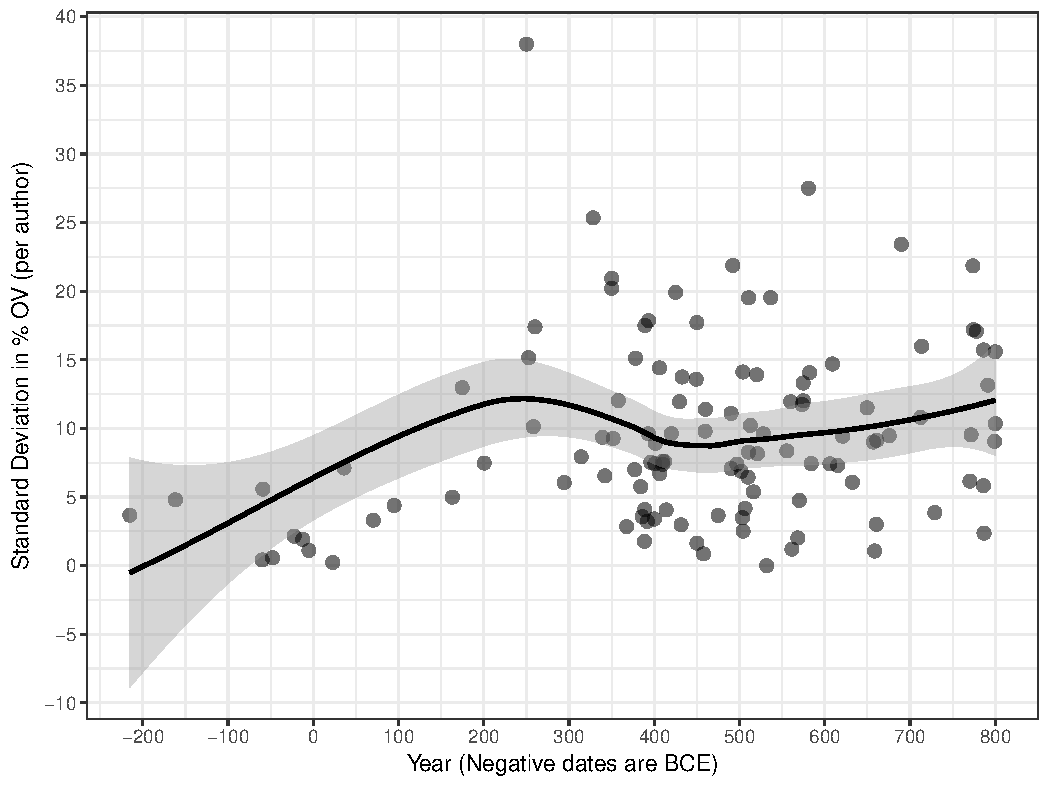
\includegraphics[width=\textwidth]{sp_authorvar.pdf}
\end{figure}
\noindent This variability of the data is also a cautionary tale. It would be easy enough, based on the complete data, to select a thousand lines of Livy and a thousand lines of Jerome, and `show' that OV\% declined from 80\% to 25\% over four hundred years. However, comparing Seneca the Elder with the \textit{Chronicles} of Sulpicius Severus would show that OV\% actually \textit{increased} over the same period. Selective sampling is always dangerous, but especially so on data with high variability.

\section{Conclusions and Future Work}

As far as I am aware, this study is by far the most comprehensive statistical survey of Latin verb order. I analysed 1178 works, spanning 1035 years and totalling 1.87 million sentences. This resulted in around half a million conclusive categorisations of sentences as OV or VO. There is still, however, a great deal of work to be performed. The greatest concern, at this stage, is that my computational results have not been independently shown to be reliable. One avenue for future work would therefore be to objectively measure, and hopefully improve, the accuracy of the automated analysis. The data, as it stands, offers many attractive avenues for further research. It would be interesting to separate the works by region, and analyse the trends separately---did word order change differently in Gaul, for example, than Spain or Italy? Single author results (for example the 98 works by Saint Jerome) could be used to make observations about pragmatics---treating OV\% as a possible component of register or style. With only moderate changes, the analysis framework could be adapted to investigate related phenomena---for example the use of the synthetic Latin passive as compared to reflexive constructions with \textit{se}.\footnote{This could extend or build on the work by \cite{green}.} I hope that, by placing the full results and methodology in the public domain, the data can be useful for future studies.

My main research aim was to find a way to collect and analyse data on a much larger scale than previous studies, not to draw conclusions. However, there are some observations from the raw data that seem interesting. The first observation is that, considering the entire period from 235\bce to 800\textsc{ce}, there is insufficient statistical evidence to support a correlation between date and OV\%. At this point it seems important to recall that we are measuring Latin as \textit{written}---it is by no means clear (and this data seems to suggest that it is false) that written works over the entirety of this period are a valid reflection of spoken language. The second observation is that there is modest evidence that OV\% declined over time up to the early fifth century \textsc{ce}. This was demonstrated using a piecewise weighted linear regression with a break at 425\textsc{ce}, indicating a downward trend with greater than 99\% confidence ($p$-value $<$\,2$\times\,\text{10}^{-\text{16}}$) and a reasonable (but not compelling) R-squared value of around 17\%. The last important finding is that, supporting \cite{pinkster}, the data displays extreme synchronic variation, both between authors and within the works of a single author. The 98 works of Saint Jerome range between 14\% and 92\% OV. This per-author variation appears to be greater in post-Classical authors. Overall this data, in isolation, offers only modest evidence in support of Latin verb-order change, even though it must have occurred. There is no evidence in the data for a strong syntactic OV order in Classical Latin. There is no evidence for a definitive OV to VO shift in written texts over the entire period, and there is only modest evidence for an OV to VO shift up to 425\textsc{ce}. The data also shows, due to its variability, the danger of comparative studies using small sample spaces---it would be extremely easy to draw misleading conclusions. Overall, while it is a historical fact that Latin underwent linguistic change, it seems that this is best supported by a combination of objective analyses (like this one) and historical and textual evidence.

\newpage
\bibliographystyle{apacite}
\bibliography{ovvo}
\end{document}
